\chapter{System Requirements}

The current chapter identifies the system requirements required for the development of the proposed QRAG system. The system combines the traditional RAG system architecture with Quantum NLP systems, which therefore requires conventional as well as quantum computing infrastructure.

\section{Functional Requirements}

The functional requirements of the system are summarized in Table~\ref{tab:functional_requirements}. These requirements define the core operations that the system must perform to ensure proper functionality.

\begin{table}[htbp]
    \centering
    \caption{Functional Requirements}
    \label{tab:functional_requirements}
    \begin{tabular}{|c|p{5cm}|p{6cm}|}
        \hline
        \textbf{ID} & \textbf{Function} & \textbf{Description} \\
        \hline
        F1 & Query Processing & Accept and preprocess user queries \\
        \hline
        F2 & Ambiguity Detection & Identify syntactic ambiguity using POS tagging \\
        \hline
        F3 & Hybrid Routing & Route queries to classical or quantum pipeline \\
        \hline
        F4 & Knowledge Graph Extraction & Dynamically extract and validate entities to populate the Neo4j database. \\
        \hline
        F5 & Constructive Hallucination & Algorithmically capture unprompted LLM entity relationships to enrich the retrieval context. \\
        \hline
        F6 & Classical Parsing & Process simple queries using SpaCy and retrieval system \\
        \hline
        F7 & Quantum Processing & Process ambiguous queries using VQC and quantum circuits \\
        \hline
        F8 & Contextual Realignment & Select correct interpretation of query \\
        \hline
        F9 & Document Retrieval & Fetch relevant documents from vector database \\
        \hline
        F10 & Response Generation & Generate final output using LLM \\
        \hline
    \end{tabular}
\end{table}

\section{Non-Functional Requirements}

The non-functional requirements define system quality attributes such as performance, reliability, and security. These are summarized in Table~\ref{tab:nonfunctional_requirements}.

\begin{table}[htbp]
    \centering
    \caption{Non-Functional Requirements}
    \label{tab:nonfunctional_requirements}
    \begin{tabular}{|c|p{5cm}|p{6cm}|}
        \hline
        \textbf{ID} & \textbf{Requirement} & \textbf{Description} \\
        \hline
        NF1 & Performance & Low latency for classical queries and acceptable delay for quantum queries \\
        \hline
        NF2 & Scalability & Ability to handle concurrent users using cloud scaling \\
        \hline
        NF3 & Reliability & Stable operation with minimal downtime \\
        \hline
        NF4 & Security & Secure API access and encrypted communication \\
        \hline
        NF5 & Maintainability & Modular architecture for easy updates \\
        \hline
        NF6 & Usability & User-friendly interface for interaction \\
        \hline
    \end{tabular}
\end{table}

\section{Hardware and Software Requirements}

The hardware and software requirements required for development and deployment are summarized in Table~\ref{tab:hardware_software}.

\begin{table}[htbp]
    \centering
    \caption{Hardware and Software Requirements}
    \label{tab:hardware_software}
    \begin{tabular}{|p{4cm}|p{8cm}|}
        \hline
        \textbf{Category} & \textbf{Specifications} \\
        \hline
        Processor & Intel i5 / AMD Ryzen 5 or higher \\
        \hline
        RAM & Minimum 8 GB (16 GB recommended) \\
        \hline
        Storage & At least 20 GB free disk space \\
        \hline
        Cloud Platform & Microsoft Azure (App Services, VM) \\
        \hline
        Backend & Python, FastAPI, Gunicorn, Uvicorn \\
        \hline
        Frontend & React.js, Tailwind CSS, Recharts \\
        \hline
        Database & MongoDB Atlas (Vector Search), Neo4j \\
        \hline
        Quantum Tools & Qiskit, lambeq, IBM Brisbane 127-qubit QPU \\
        \hline
        NLP Tools & SpaCy, Transformer-based embeddings \\
        \hline
    \end{tabular}
\end{table}

\section{System Architecture Requirements}

Modular and decoupled architecture has been used for scalability and maintainability purposes. The architecture enables both the classic and quantum pipeline to work independently but still maintains effective communication within the different system components.

\begin{itemize}
    \item RESTful API communication between frontend and backend
    \item Separation of classical and quantum pipelines
    \item Integration layer for combining retrieval and generation
    \item Asynchronous request handling
\end{itemize}

\section{Deployment Requirements}

The QRAG system is deployed using a cloud-native architecture. The deployment configuration and infrastructure setup are illustrated in Figures~\ref{fig:deployment_1} to \ref{fig:deployment_5}.

\begin{itemize}
    \item Backend deployed using Gunicorn with Uvicorn workers on dedicated Azure App Services (e.g., ragqrag-backend)
    \item Frontend served via PM2 and routed through a dedicated .tech custom domain for production research evaluation
    \item Lazy loading of models to reduce startup time
    \item Container timeout handling
    \item CORS configuration for secure communication between the frontend domain and the Azure backend
\end{itemize}

Figure~\ref{fig:deployment_1} and Figure~\ref{fig:deployment_2} show the initial deployment configurations and service setup within the Azure environment.

\begin{figure}[htbp]
    \centering
    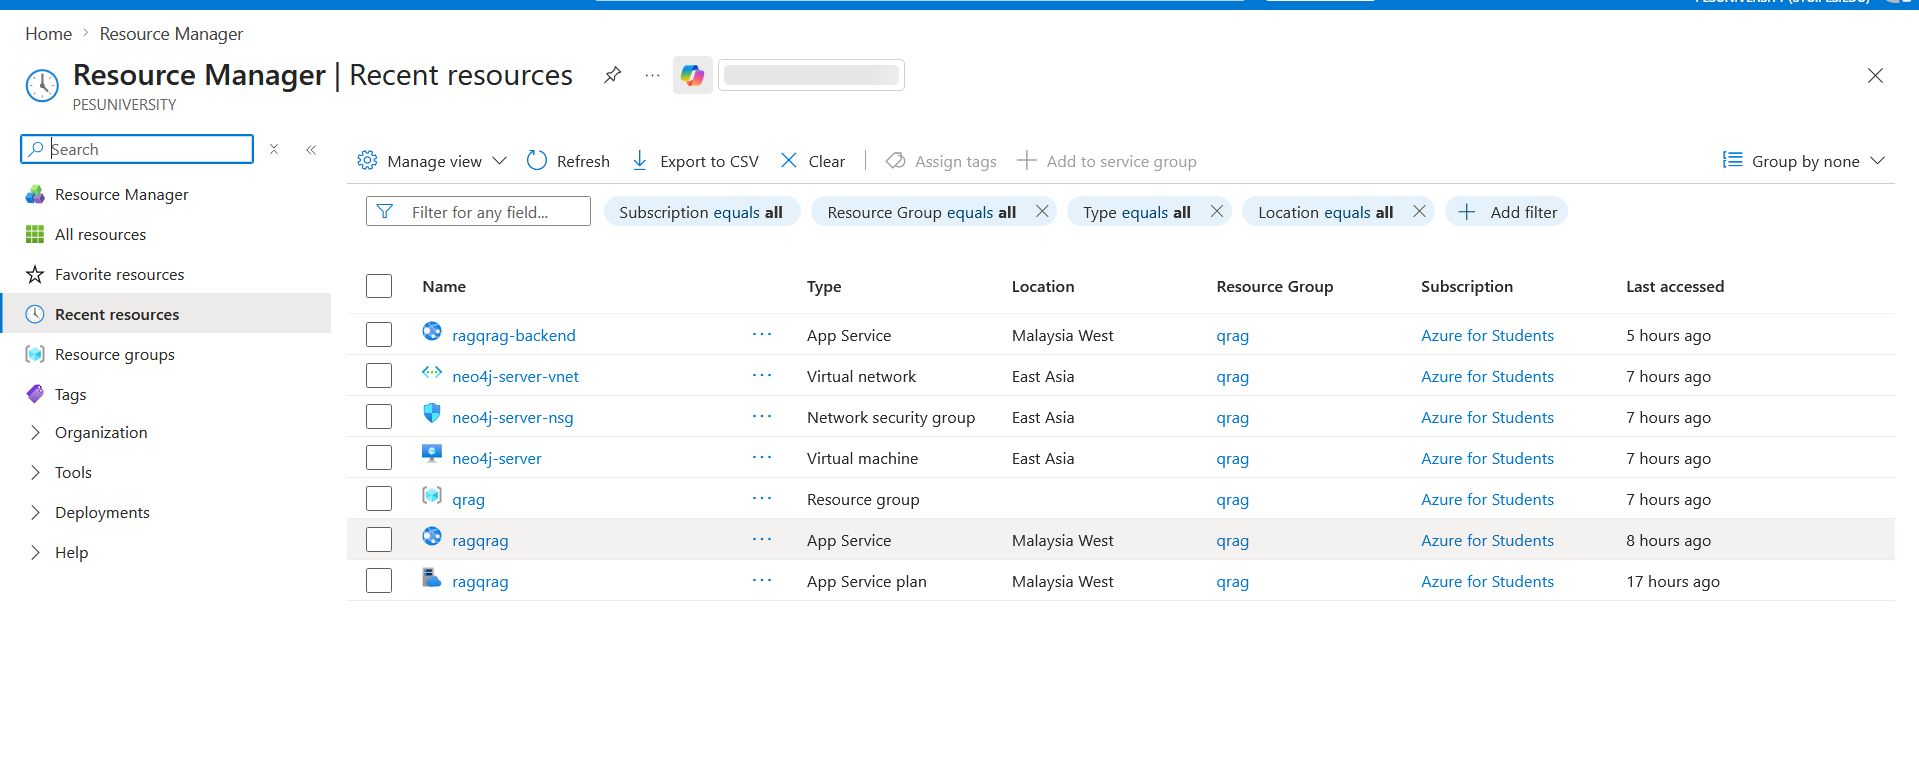
\includegraphics[width=0.8\textwidth]{assets/deployment/Screenshot 2026-04-02 162800.png}
    \caption{Azure deployment resources overview.}
    \label{fig:deployment_1}
\end{figure}

\begin{figure}[htbp]
    \centering
    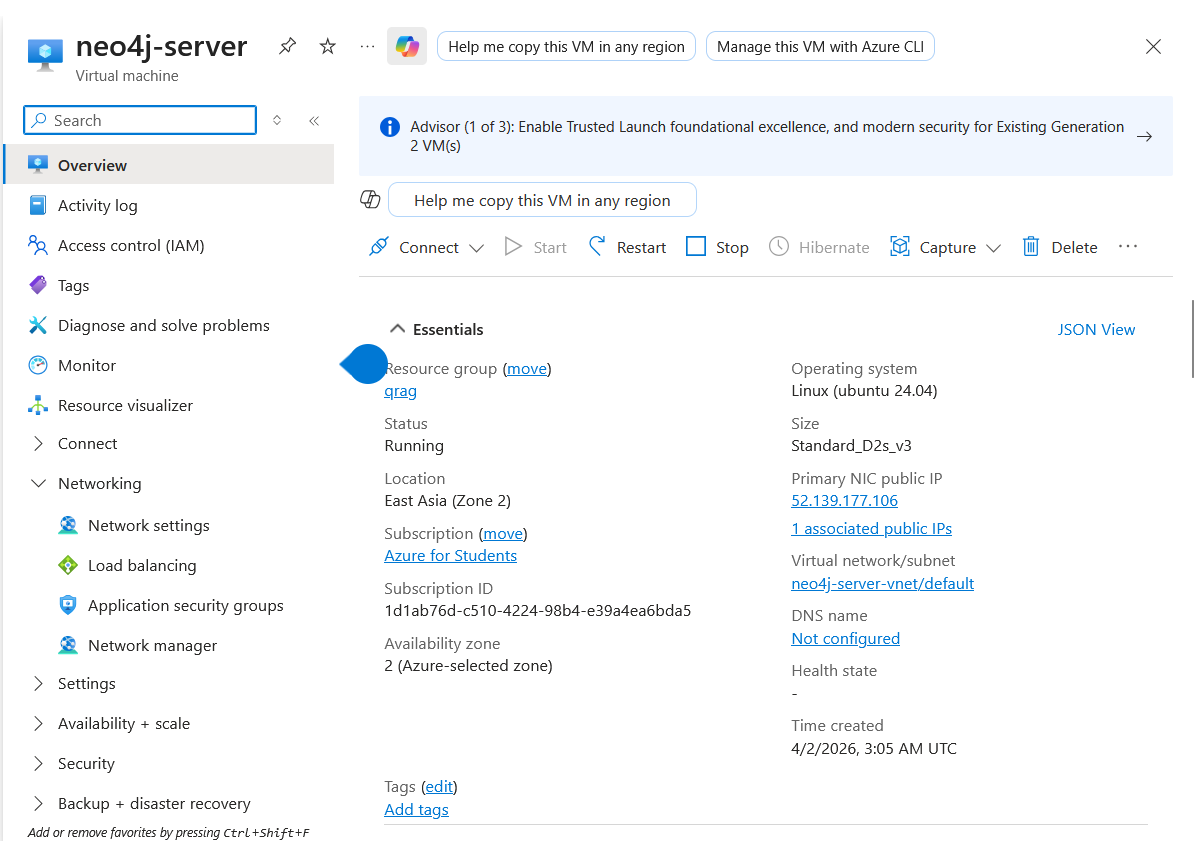
\includegraphics[width=0.8\textwidth]{assets/deployment/Screenshot 2026-04-02 162816.png}
    \caption{Azure resource grouping and service configuration.}
    \label{fig:deployment_2}
\end{figure}

Further configuration details and runtime logs are presented in Figure~\ref{fig:deployment_3} and Figure~\ref{fig:deployment_4}, highlighting backend deployment and service execution.

\begin{figure}[htbp]
    \centering
    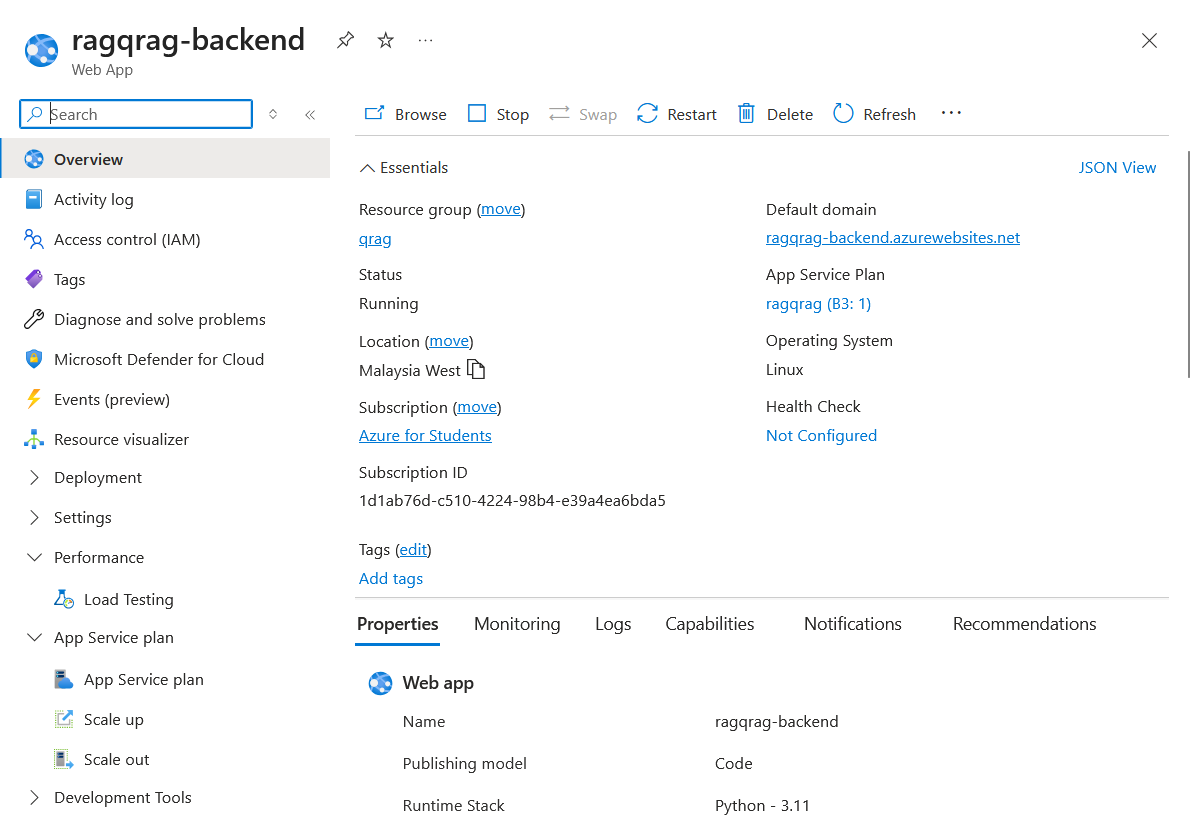
\includegraphics[width=0.8\textwidth]{assets/deployment/Screenshot 2026-04-02 162900.png}
    \caption{Backend deployment logs and service execution.}
    \label{fig:deployment_3}
\end{figure}

\begin{figure}[htbp]
    \centering
    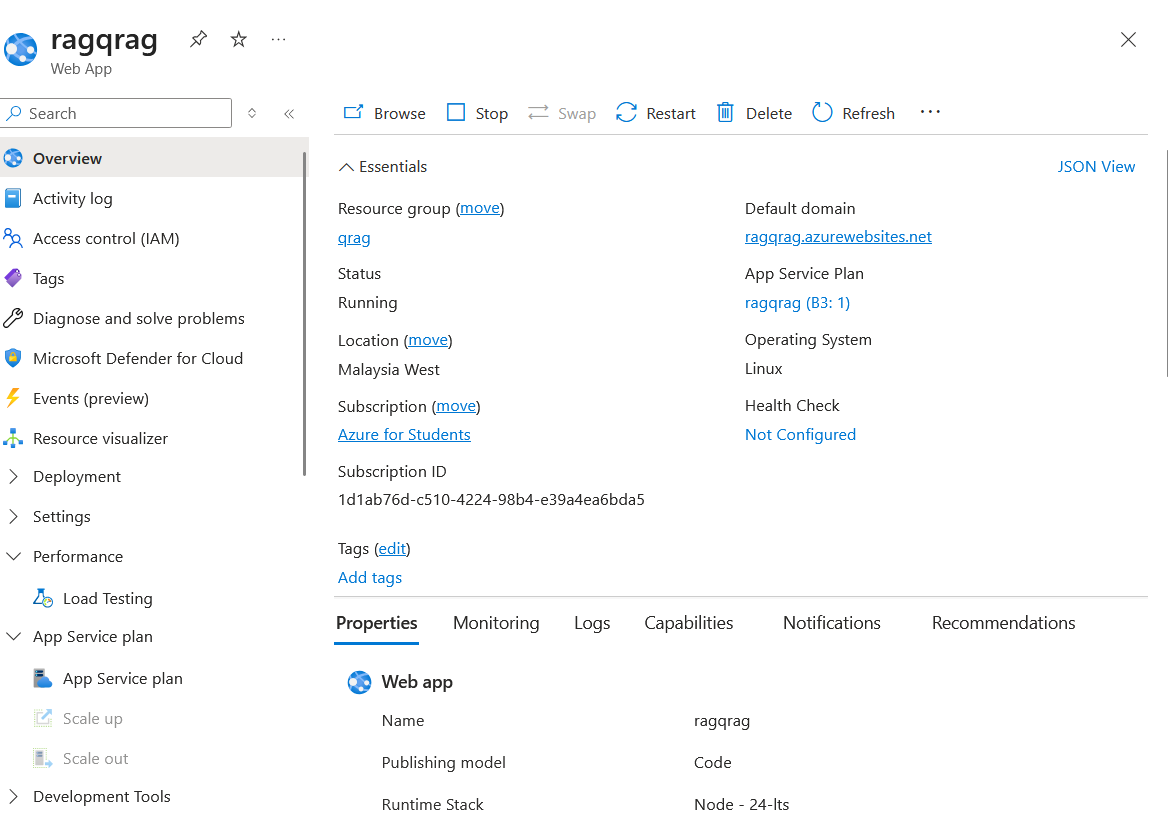
\includegraphics[width=0.8\textwidth]{assets/deployment/Screenshot 2026-04-02 162913.png}
    \caption{Application runtime monitoring and configuration.}
    \label{fig:deployment_4}
\end{figure}

The complete deployment topology and cloud architecture are shown in Figure~\ref{fig:deployment_5}, demonstrating the integration of frontend, backend, and database services.

\begin{figure}[htbp]
    \centering
    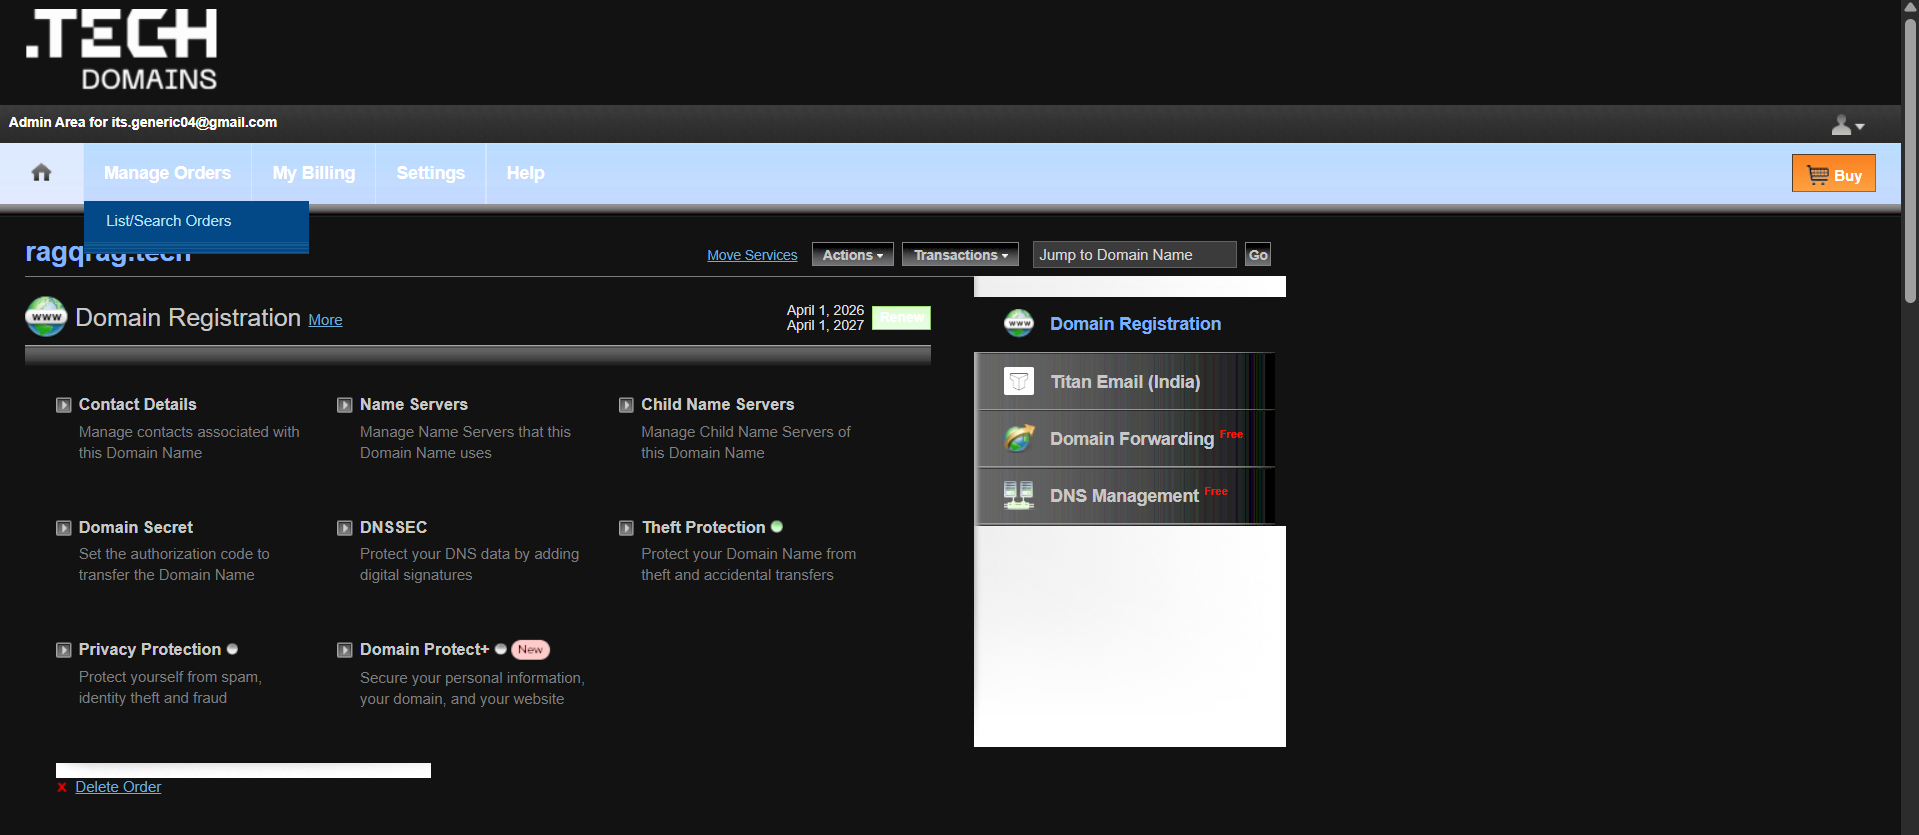
\includegraphics[width=0.85\textwidth]{assets/deployment/Screenshot 2026-04-03 133517.png}
    \caption{Overall deployment architecture and system topology.}
    \label{fig:deployment_5}
\end{figure}

\section{Performance and Security Requirements}

\textbf{Performance:}
\begin{itemize}
    \item Low latency for classical processing pipeline
    \item Controlled latency for quantum processing
    \item Efficient vector-based retrieval
\end{itemize}

\textbf{Security:}
\begin{itemize}
    \item Secure API endpoints
    \item Encrypted database communication
    \item HTTPS-based communication across services
\end{itemize}

\section{Scalability and Optimization}

The system is designed to support scalability and efficient resource utilization through cloud-native practices.

\begin{itemize}
    \item Dynamic scaling of Azure services (B1 to P1v3 tiers)
    \item Cost optimization through selective quantum usage
    \item Separation of compute-intensive workloads
\end{itemize}

\bigskip\noindent
The system requirements ensure that the framework operates efficiently while maintaining scalability, reliability, and performance. The hybrid infrastructure supports both classical and quantum components effectively.
